\documentclass{article}
\usepackage[utf8]{inputenc}
\usepackage{graphicx}
\usepackage{geometry}
\geometry{a4paper, margin=1in}
\usepackage{amsmath}
\usepackage{hyperref}
\usepackage{float}
\usepackage{listings}
\usepackage{xcolor}

\definecolor{codegreen}{rgb}{0,0.6,0}
\definecolor{codegray}{rgb}{0.5,0.5,0.5}
\definecolor{codepurple}{rgb}{0.58,0,0.82}
\definecolor{backcolour}{rgb}{0.95,0.95,0.92}

\lstdefinestyle{mystyle}{
    backgroundcolor=\color{backcolour},   
    commentstyle=\color{codegreen},
    keywordstyle=\color{magenta},
    numberstyle=\tiny\color{codegray},
    stringstyle=\color{codepurple},
    basicstyle=\ttfamily\footnotesize,
    breakatwhitespace=false,         
    breaklines=true,                 
    captionpos=b,                    
    keepspaces=true,                 
    numbers=left,                    
    numbersep=5pt,                  
    showspaces=false,                
    showstringspaces=false,
    showtabs=false,                  
    tabsize=2
}
\lstset{style=mystyle}

\title{SPICE Exercises Progress Report}
\author{Getting Ready for my PhD!}
\date{\today}

\begin{document}

\maketitle

\section*{Introduction}
I've put together this report to track my progress on the SPICE exercises suggested by Prof. Sunil Khatri (Texas A\&M). The goal is to get myself completely comfortable with SPICE before starting my PhD next year. Here, I'm documenting the key learnings and simulations I've run so far, mainly focusing on Cadence Spectre.

\section{Control Statements}
I started by getting a handle on control statements in Spectre. It's pretty cool how I can dynamically change parameters on the fly without restarting the whole simulator.

\subsection{Dynamic Parameter Modification (\texttt{alter})}
I used the \texttt{alter} statement to change the temperature between distinct analysis runs. 
\begin{lstlisting}[language=C, caption=Spectre Alter Statement Example]
// DC analysis at nominal temperature
dc1 dc oppoint=logfile homotopy=gmin 

// Change temperature and run transient analysis
Change1 alter param=temp value=100
tran1 tran stop=1u
\end{lstlisting}

\begin{figure}[H]
    \centering
    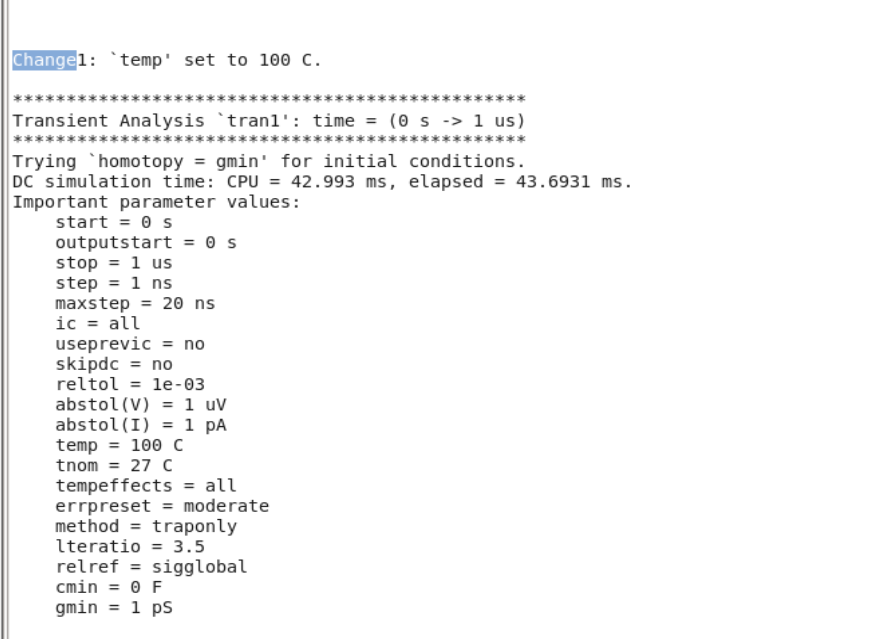
\includegraphics[width=0.8\textwidth]{SPECTRE/Control_statements/change_in_temperature_parameter_via_alter_statement.png}
    \caption{Changing temperature via alter statement.}
\end{figure}

\subsection{Output Data Extraction (\texttt{info})}
I figured out how to extract specific component parameters using the \texttt{info} statement and route it straight to my logfile.
\begin{figure}[H]
    \centering
    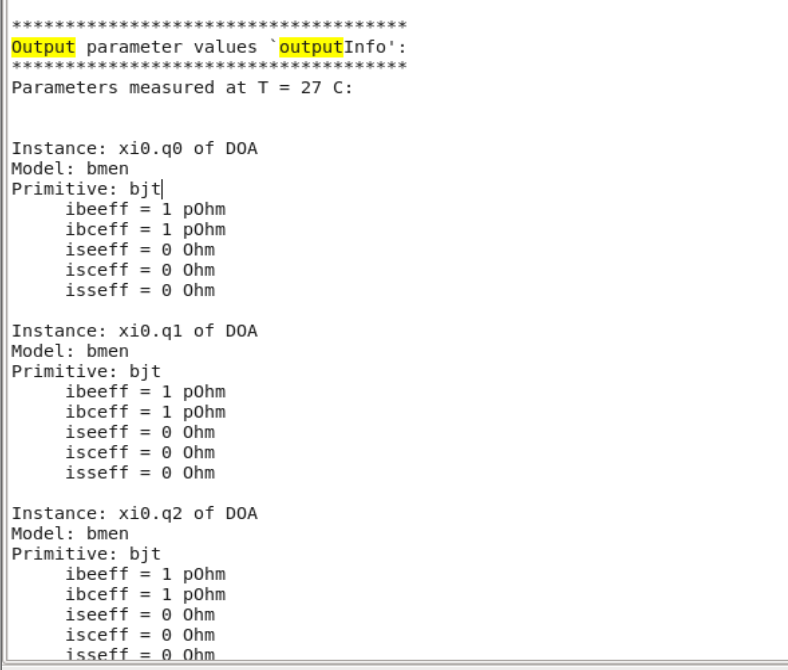
\includegraphics[width=0.8\textwidth]{SPECTRE/Control_statements/use_of_info_control_statement.png}
    \caption{Routing specific output data to the logfile.}
\end{figure}

\subsection{Profiling Performance (\texttt{simstat})}
By setting \texttt{simstat=detailed}, I was able to get an in-depth breakdown of memory usage and CPU time. This will definitely be handy for larger simulations during my PhD.
\begin{figure}[H]
    \centering
    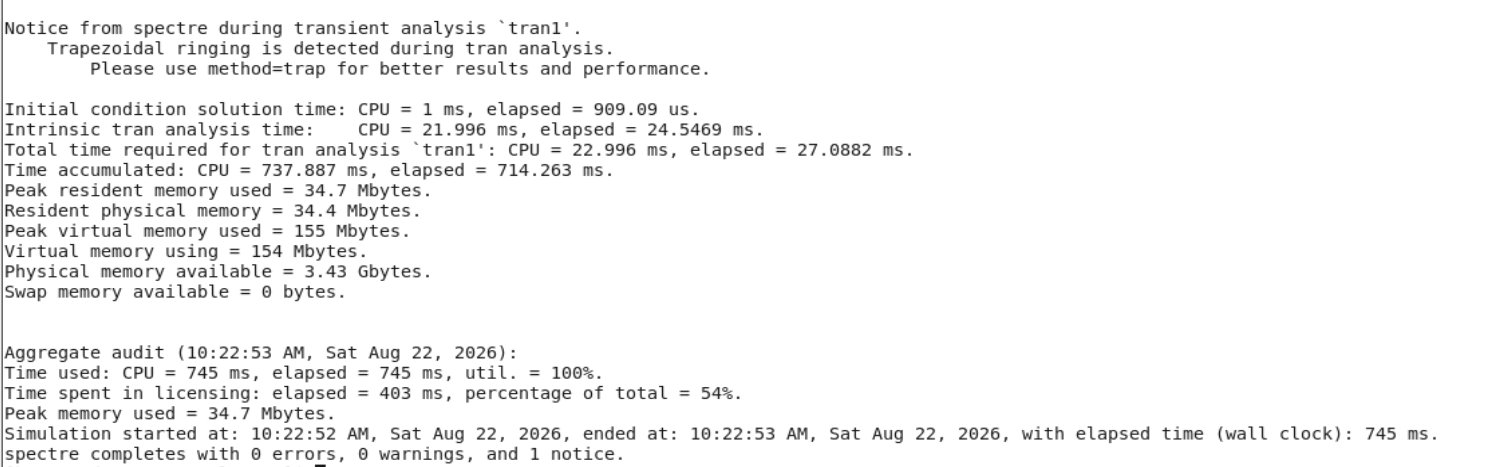
\includegraphics[width=0.8\textwidth]{SPECTRE/Control_statements/simstat_detailed_output.png}
    \caption{Detailed simstat output for performance profiling.}
\end{figure}

\section{Temperature vs Trise}
Next, I dug into how temperature is handled in device models. There's a fundamental difference between \texttt{temp} and \texttt{trise} that I needed to clarify for myself. 

I found that \texttt{temp} is \textbf{exclusive} (it overrides ambient settings) whereas \texttt{trise} is \textbf{accumulative} (it adds on top of the ambient temperature).

\begin{figure}[H]
    \centering
    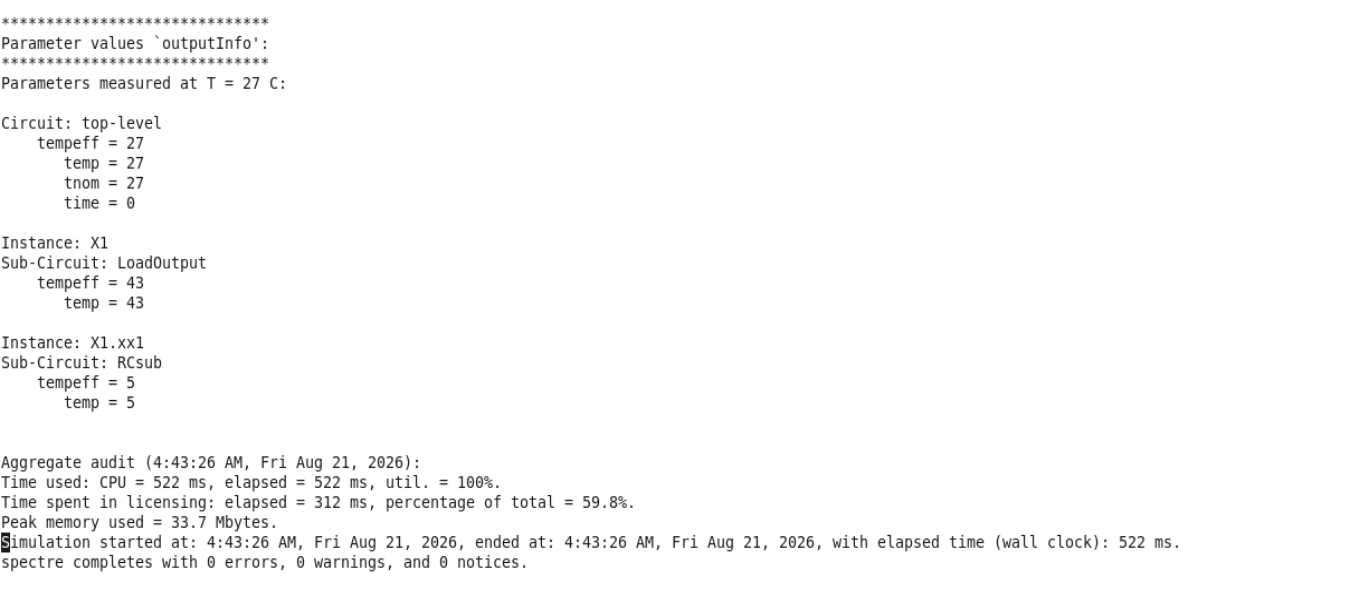
\includegraphics[width=0.8\textwidth]{SPECTRE/temp_vs_trise/temp_command_exclusive_temperature.png}
    \caption{Exclusive nature of the temp parameter.}
\end{figure}

\begin{figure}[H]
    \centering
    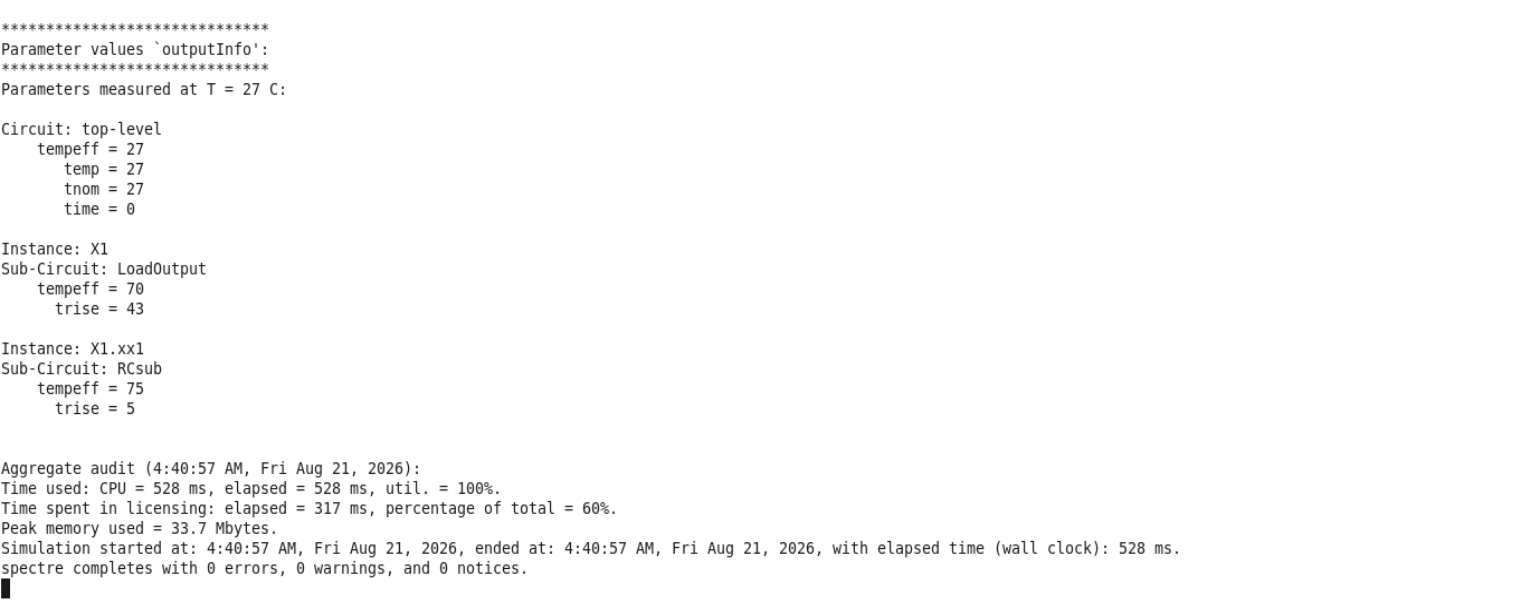
\includegraphics[width=0.8\textwidth]{SPECTRE/temp_vs_trise/trise_accumulative_effect_demo.png}
    \caption{Accumulative nature of the trise parameter.}
\end{figure}

\begin{figure}[H]
    \centering
    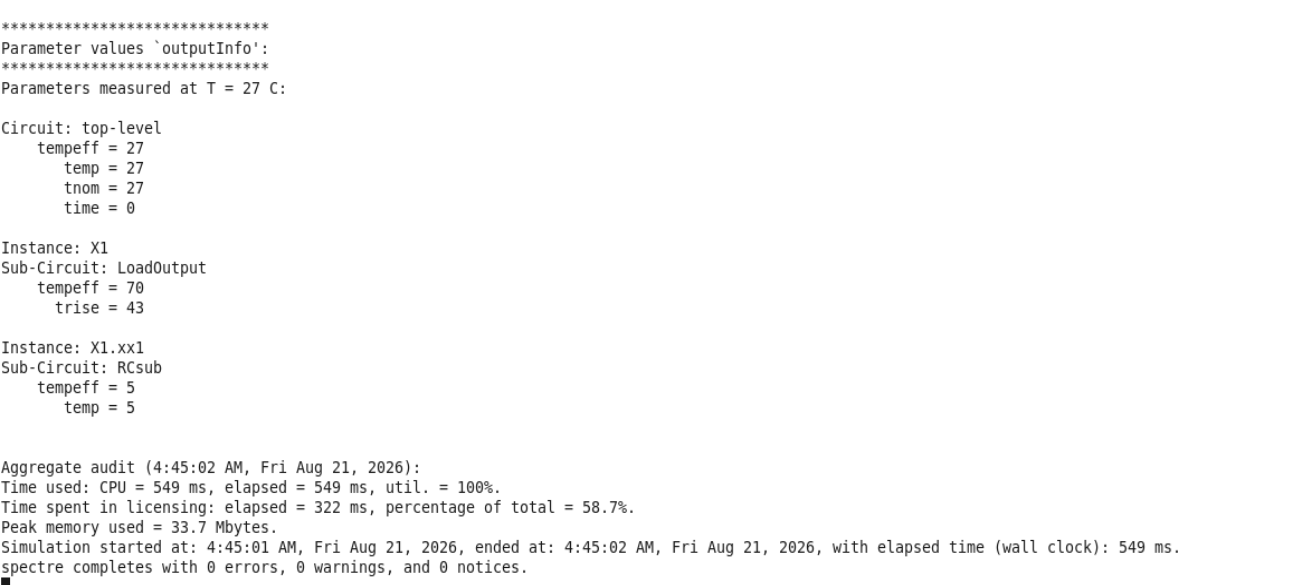
\includegraphics[width=0.8\textwidth]{SPECTRE/temp_vs_trise/demo_showing_accumulative_nature_of_trise_and_exclusive_nature_of_temp_same_time.png}
    \caption{Combined effect: trise accumulates while temp acts exclusively.}
\end{figure}


\section{Exercise 1: CMOS Inverter Chain}
For the first formal exercise, I simulated a 7-stage CMOS inverter chain using the 22-nm PTM HP model. 

\subsection{Initial Smoke Test ($k=2$)}
For my initial smoke test, I set $L = 22\text{ nm}$, $W_n = 44\text{ nm}$, $W_p = 88\text{ nm}$, and $V_{DD} = 1\text{ V}$. Measuring graphically at the 50\% $V_{DD}$ crossing, I got:
\begin{itemize}
    \item $t_{PHL} \approx 1.9286\text{ ps}$
    \item $t_{PLH} \approx 2.668\text{ ps}$
\end{itemize}
Clearly, $t_{PLH} > t_{PHL}$.

\begin{figure}[H]
    \centering
    \begin{minipage}{0.45\textwidth}
        \centering
        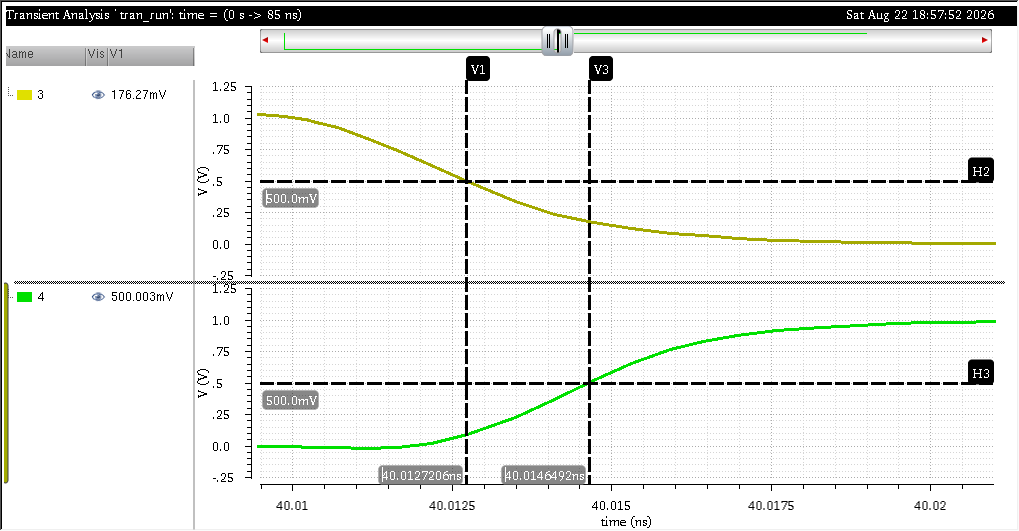
\includegraphics[width=\textwidth]{SPECTRE/Exercise1/TPHL_INVERTER_CHAIN_K_IS_2.png}
        \caption{$t_{PHL}$ measurement for $k=2$.}
    \end{minipage}\hfill
    \begin{minipage}{0.45\textwidth}
        \centering
        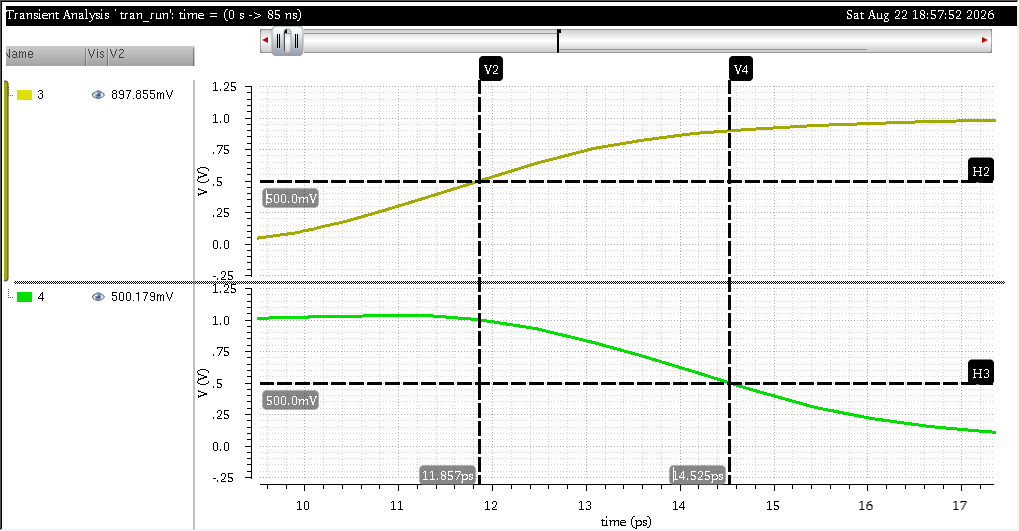
\includegraphics[width=\textwidth]{SPECTRE/Exercise1/TPLH_INVERTER_CHAIN_K_IS_2.png}
        \caption{$t_{PLH}$ measurement for $k=2$.}
    \end{minipage}
\end{figure}

\subsection{Part A: Sweep of $k$}
I wanted to find the exact PMOS-to-NMOS width ratio ($k$) where $t_{PHL} = t_{PLH}$. So, I swept $k$ from 1 to 2 in steps of 0.1.

\begin{figure}[H]
    \centering
    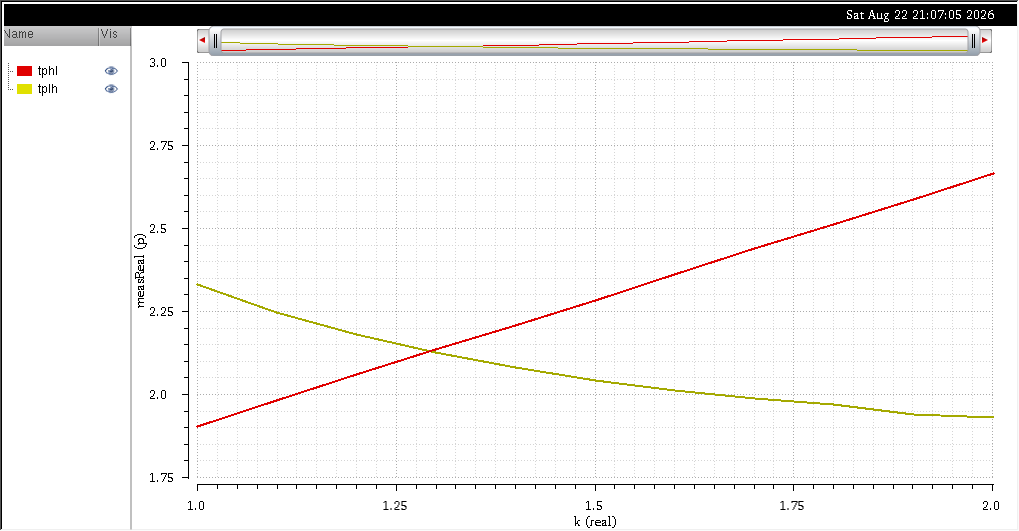
\includegraphics[width=0.8\textwidth]{SPECTRE/Exercise1/tplh_vs_tphl_as_a_function_of_k.png}
    \caption{Sweep result showing $t_{PLH}$ and $t_{PHL}$ as a function of $k$.}
\end{figure}

From my sweep data, the curves intersect around $k \approx 1.293$, where $t_{PHL} \approx t_{PLH} \approx 2.13\text{ ps}$. I verified this using the Spectre calculator, which gave me the exact same intersection point.

\begin{figure}[H]
    \centering
    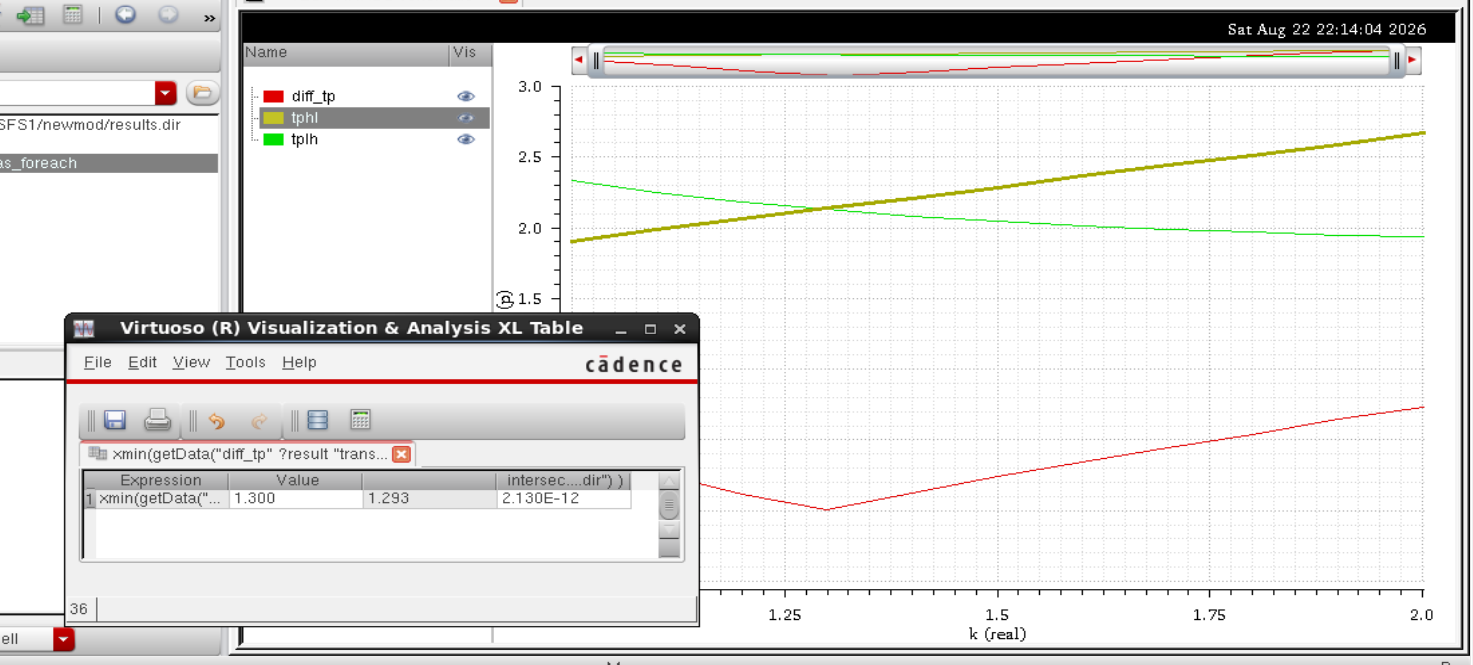
\includegraphics[width=0.8\textwidth]{SPECTRE/Exercise1/k_value_for_tplh_equal_tphl_from_calc_utility.png}
    \caption{Spectre calculator utility confirming $k \approx 1.293$.}
\end{figure}

I also looked at the rise and fall times ($t_{rise}$ and $t_{fall}$) over the same $k$ sweep. These two intersect at a different point than the propagation delays.

\begin{figure}[H]
    \centering
    \begin{minipage}{0.45\textwidth}
        \centering
        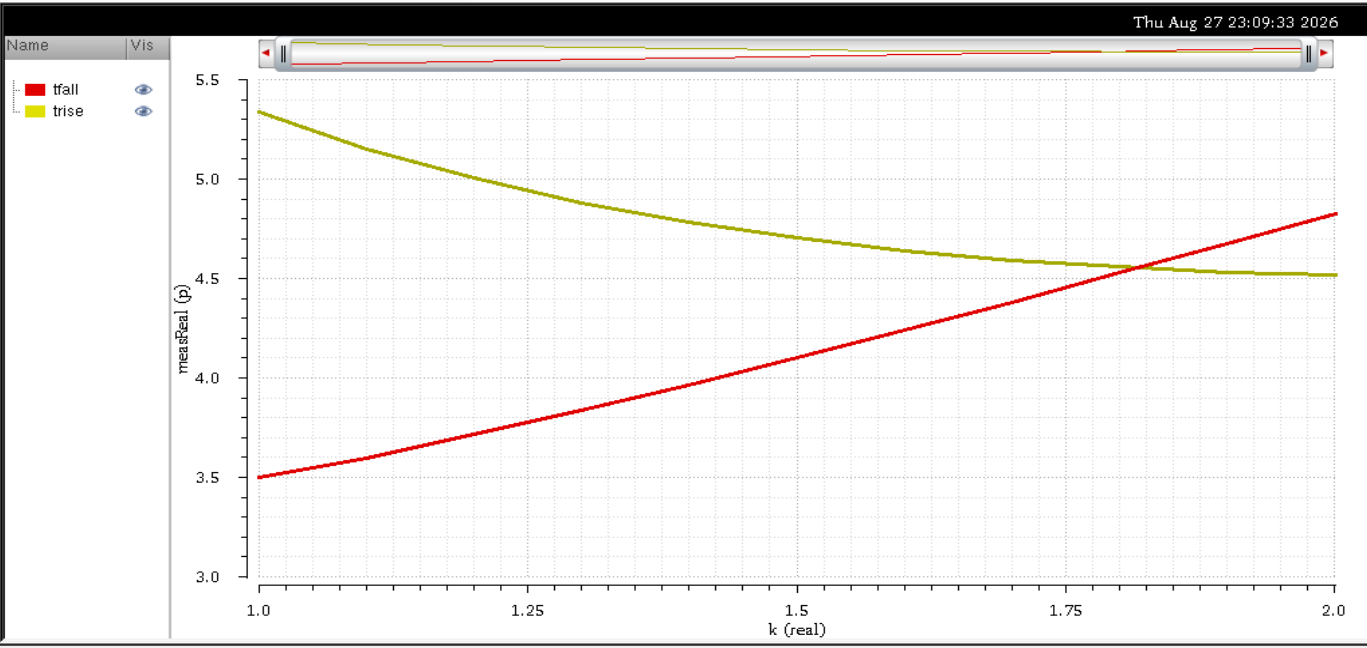
\includegraphics[width=\textwidth]{SPECTRE/Exercise1/trise_vs_tfall_values_as_k_is_swept_at_x_of10p.png}
        \caption{Spectre result: $t_{rise}$ vs $t_{fall}$ as $k$ is swept.}
    \end{minipage}\hfill
    \begin{minipage}{0.45\textwidth}
        \centering
        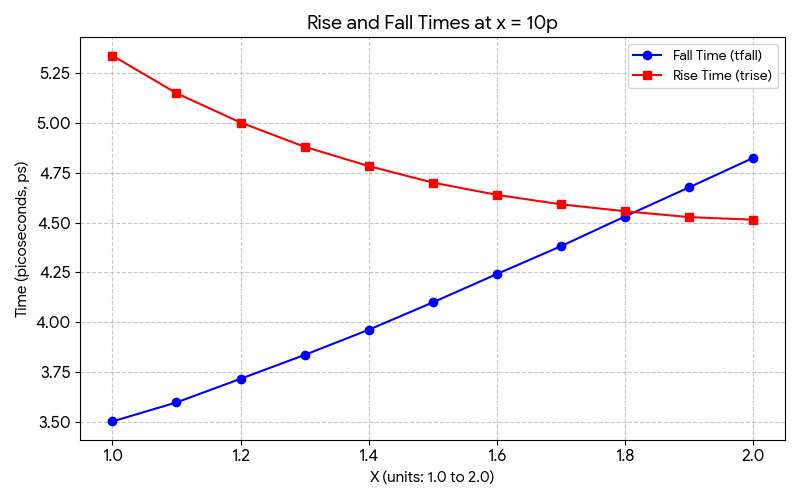
\includegraphics[width=\textwidth]{SPECTRE/Exercise1/trise_vs_tfall_python_generated.png}
        \caption{Python-generated plot of $t_{rise}$ vs $t_{fall}$.}
    \end{minipage}
\end{figure}

The rise and fall times become equal at $k \approx 1.82$, where $t_{rise} \approx t_{fall} \approx 4.55\text{ ps}$.

\subsection{Part B: Sweep of $X$ for Symmetric Rise/Fall Times}
Next, I wanted to find the input transition time ($X$) that makes $t_{rise} = t_{fall}$. I varied $X$ while keeping $k$ fixed and measured both rise and fall times.

\begin{figure}[H]
    \centering
    \begin{minipage}{0.45\textwidth}
        \centering
        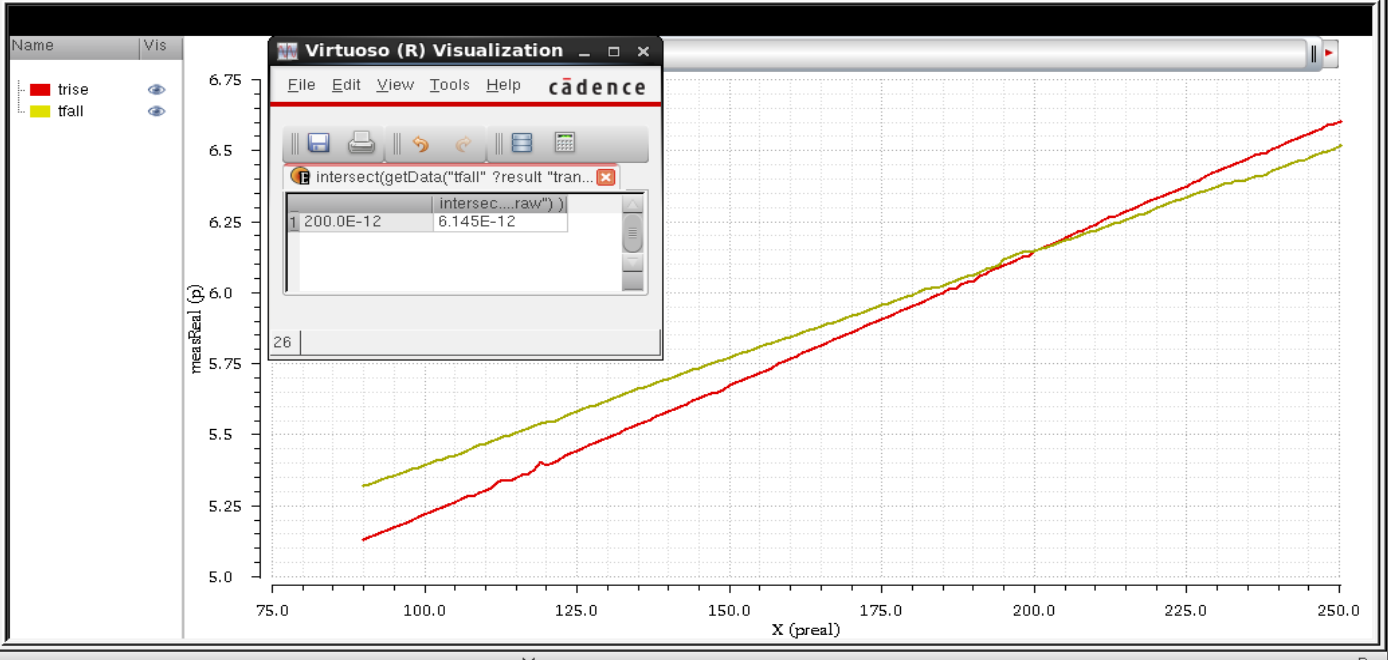
\includegraphics[width=\textwidth]{SPECTRE/Exercise1/viva_trise_tfall_as_X_is_varied_with_their_intersection_graphically_and_calculator_utility.png}
        \caption{Spectre result and calculator utility showing $t_{rise}$ vs $t_{fall}$ as $X$ is varied.}
    \end{minipage}\hfill
    \begin{minipage}{0.45\textwidth}
        \centering
        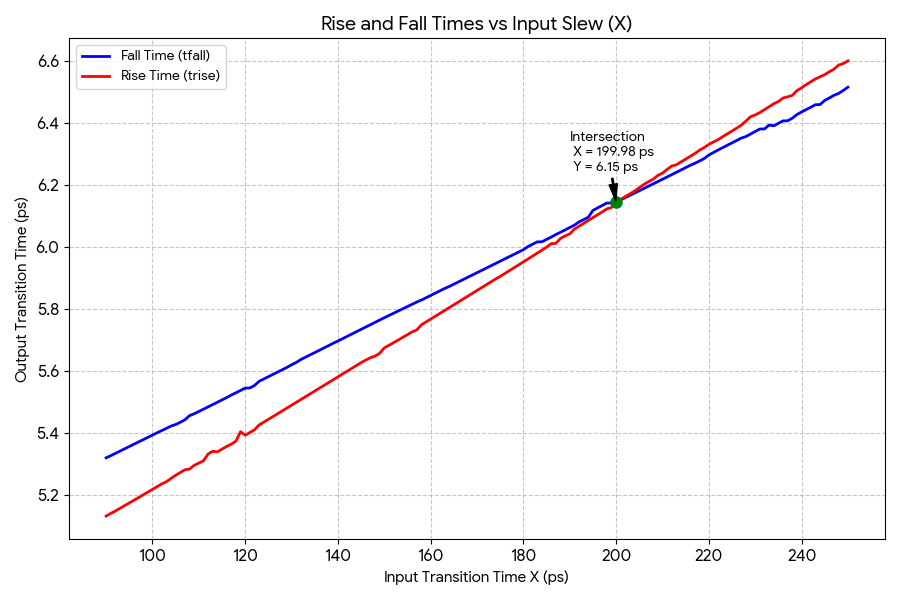
\includegraphics[width=\textwidth]{SPECTRE/Exercise1/trise_and_tfall_as_x_is_varied_python_generated.png}
        \caption{Python-generated plot of $t_{rise}$ vs $t_{fall}$ as $X$ is varied.}
    \end{minipage}
\end{figure}

The two curves intersect at $X \approx 200\text{ ps}$, giving $t_{rise} \approx t_{fall} \approx 6.145\text{ ps}$. This is the symmetric input transition time I'll use going forward.

\subsection{Part C: Sweep of $k$ at Symmetric $X$}
With the symmetric $X \approx 200\text{ ps}$ from Part B in hand, I swept $k$ again (this time from 1 to 5) to re-examine both the propagation delays and the rise/fall times.

\subsubsection{$t_{PHL}$ vs $t_{PLH}$}

\begin{figure}[H]
    \centering
    \begin{minipage}{0.45\textwidth}
        \centering
        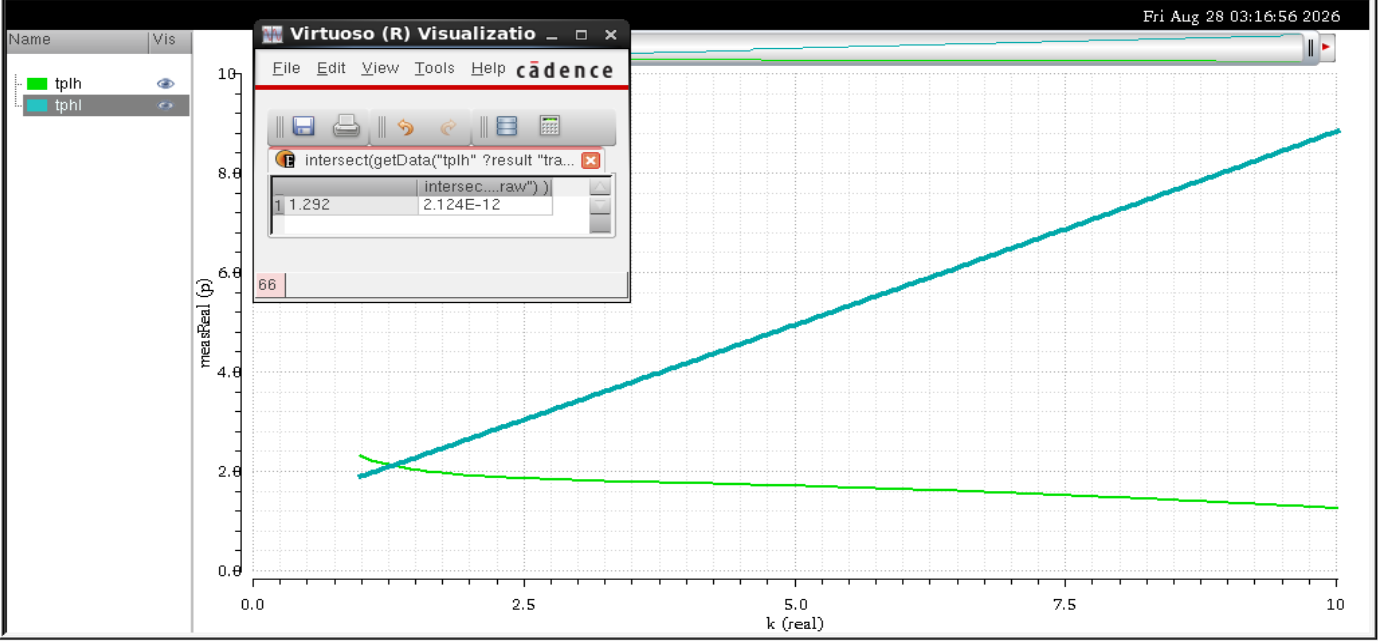
\includegraphics[width=\textwidth]{SPECTRE/Exercise1/tplh_vs_tphl_as_k_swept_for_x_at_200.png}
        \caption{Spectre result: $t_{PHL}$ vs $t_{PLH}$ at $X = 200\text{ ps}$.}
    \end{minipage}\hfill
    \begin{minipage}{0.45\textwidth}
        \centering
        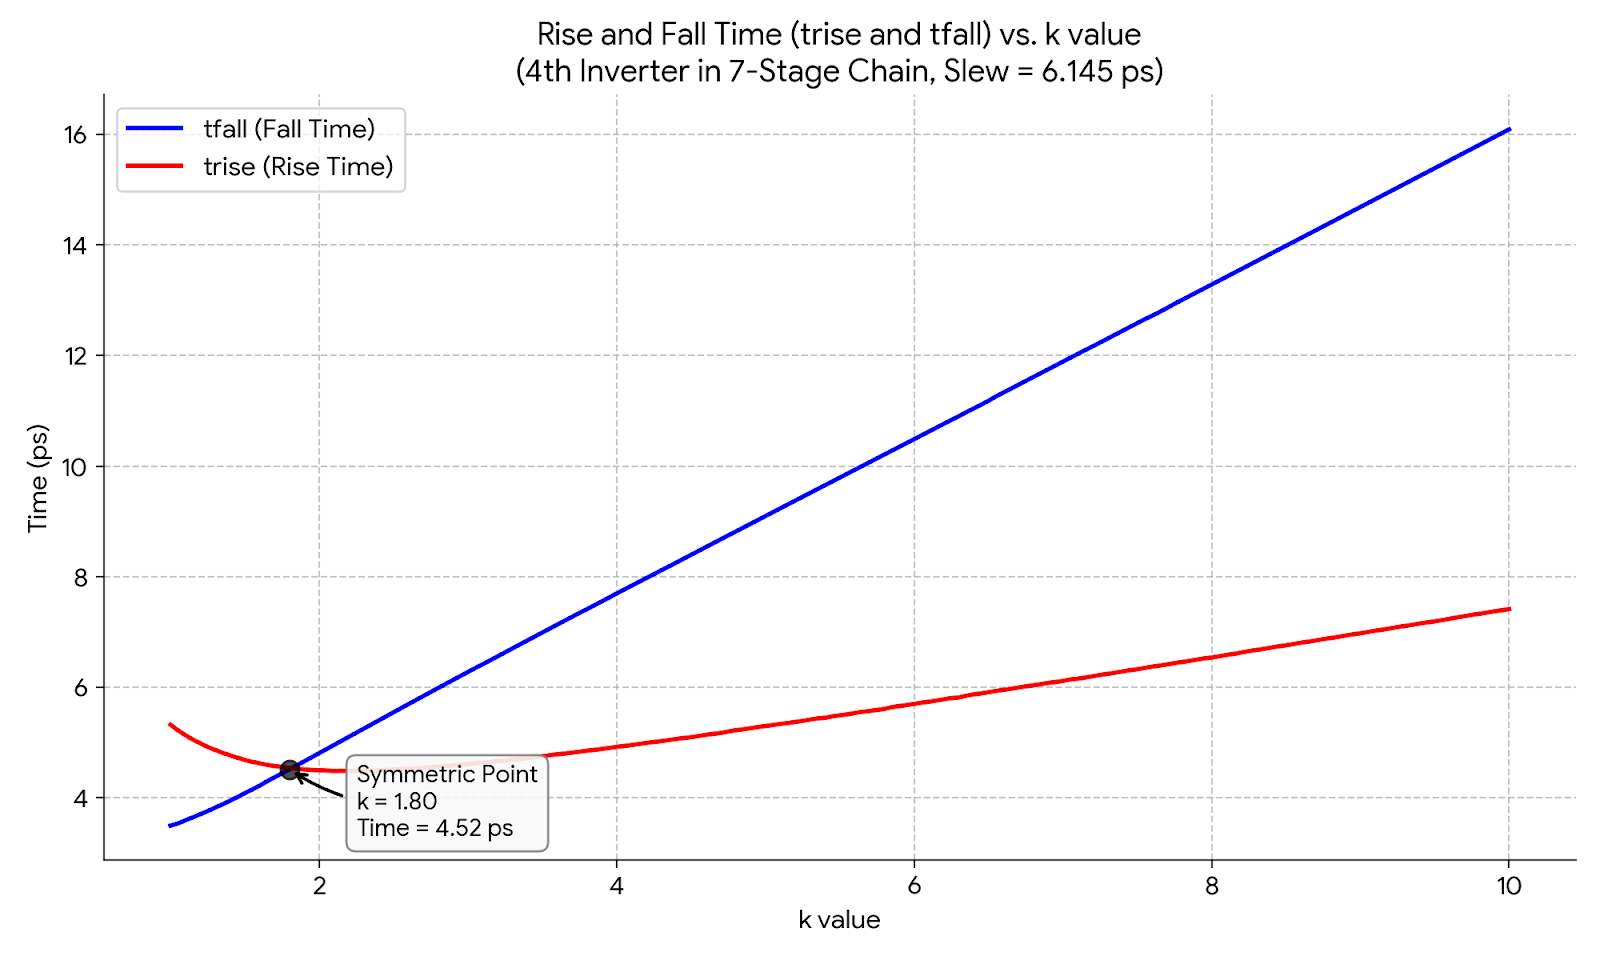
\includegraphics[width=\textwidth]{SPECTRE/Exercise1/partc_tphl_vs_tplh_as_k_is_varied_python_at_symmetric_X.png}
        \caption{Python-generated plot of $t_{PHL}$ vs $t_{PLH}$ at symmetric $X$.}
    \end{minipage}
\end{figure}

The propagation delays are now equal at $k \approx 1.38$, with $t_{PHL} \approx t_{PLH} \approx 2.45\text{ ps}$. Interestingly, this is a slightly different $k$ than Part A ($k \approx 1.293$), which makes sense since the input transition time affects the switching behavior.

\subsubsection{$t_{rise}$ vs $t_{fall}$}

\begin{figure}[H]
    \centering
    \begin{minipage}{0.45\textwidth}
        \centering
        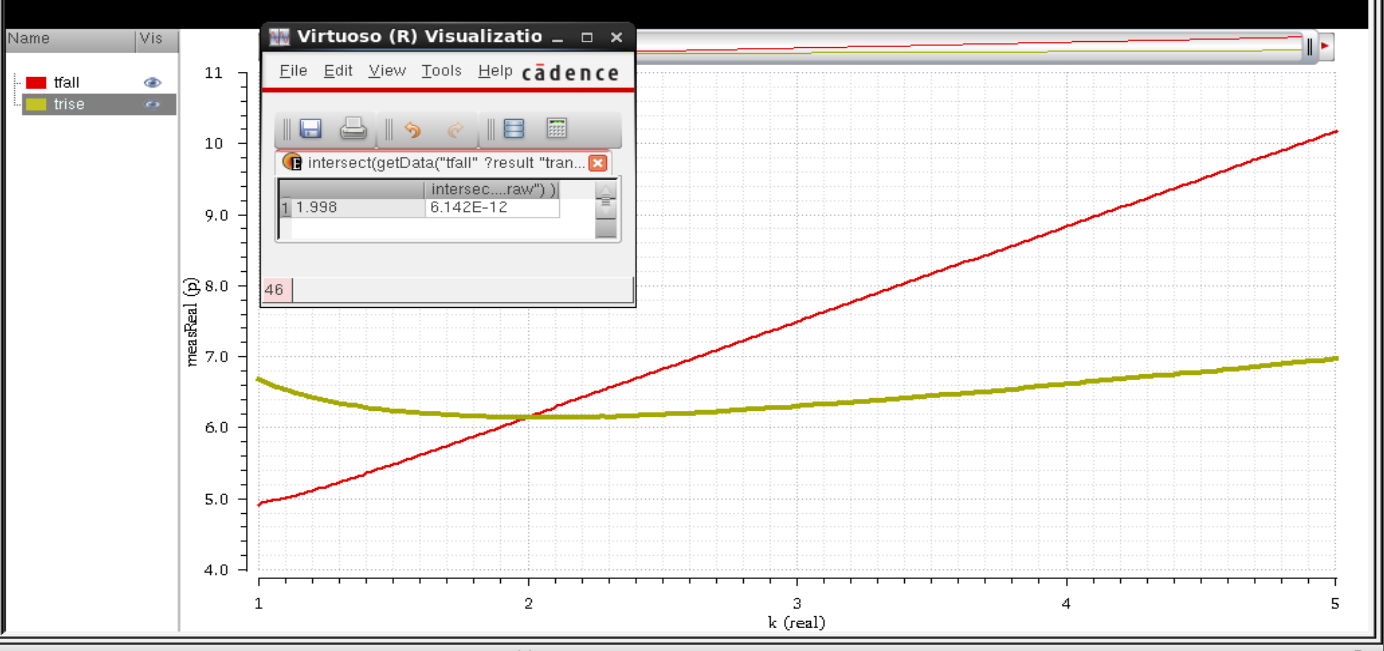
\includegraphics[width=\textwidth]{SPECTRE/Exercise1/trise_vs_tfall_as_k_swept_for_x_at_200.png}
        \caption{Spectre result: $t_{rise}$ vs $t_{fall}$ at $X = 200\text{ ps}$.}
    \end{minipage}\hfill
    \begin{minipage}{0.45\textwidth}
        \centering
        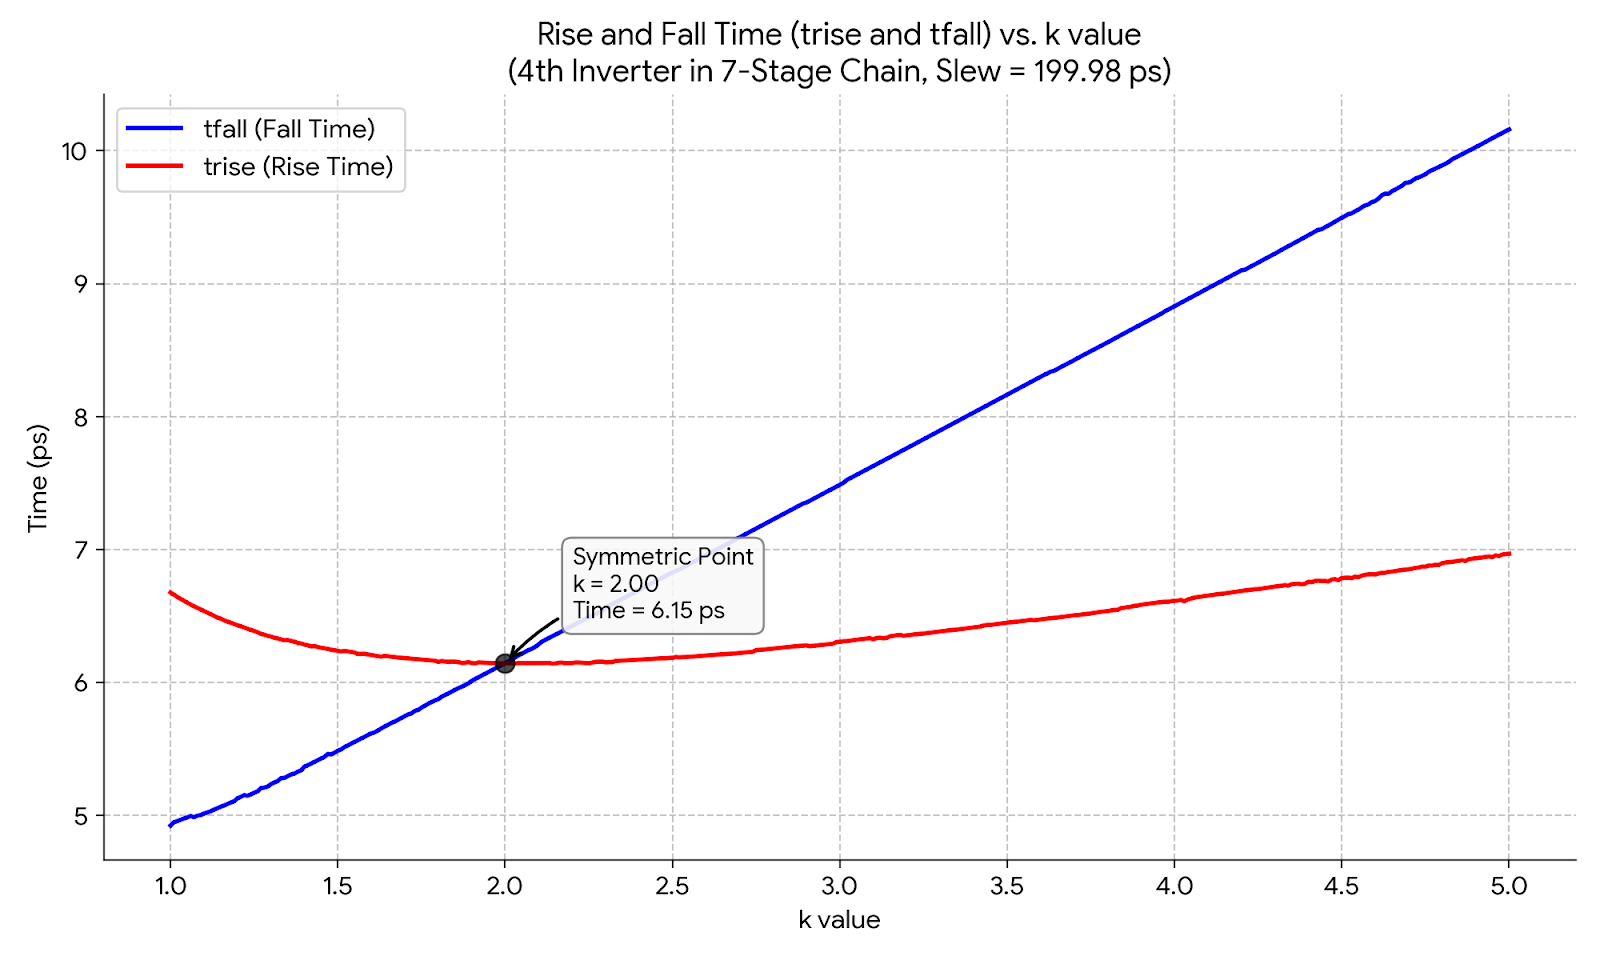
\includegraphics[width=\textwidth]{SPECTRE/Exercise1/python_partc_tr_vs_tf_t_X_symmetric_value_vs_k.png}
        \caption{Python-generated plot of $t_{rise}$ vs $t_{fall}$ at symmetric $X$.}
    \end{minipage}
\end{figure}

Here, the rise and fall times intersect at $k \approx 2.0$, with $t_{rise} \approx t_{fall} \approx 6.14\text{ ps}$.

\section*{Conclusion}
I'm making solid progress through Prof. Khatri's exercises. Getting hands-on with Spectre's control statements and understanding the nuances of the simulator will definitely pay off during my PhD research!

\end{document}
